\documentclass[tikz,border=0pt]{standalone}
\usepackage[american]{circuitikz}
\usetikzlibrary{arrows.meta,calc,positioning,decorations.pathmorphing,patterns}
\definecolor{zyloTeal}{HTML}{174A5B}
\definecolor{zyloTealTwo}{HTML}{246B7A}
\definecolor{zyloInk}{HTML}{1F2933}
\definecolor{zyloSoft}{HTML}{EAF4F4}
\definecolor{zyloPaper}{HTML}{F8FAFB}
\definecolor{zyloLine}{HTML}{44606B}
\definecolor{zyloOrange}{HTML}{D97706}
\begin{document}
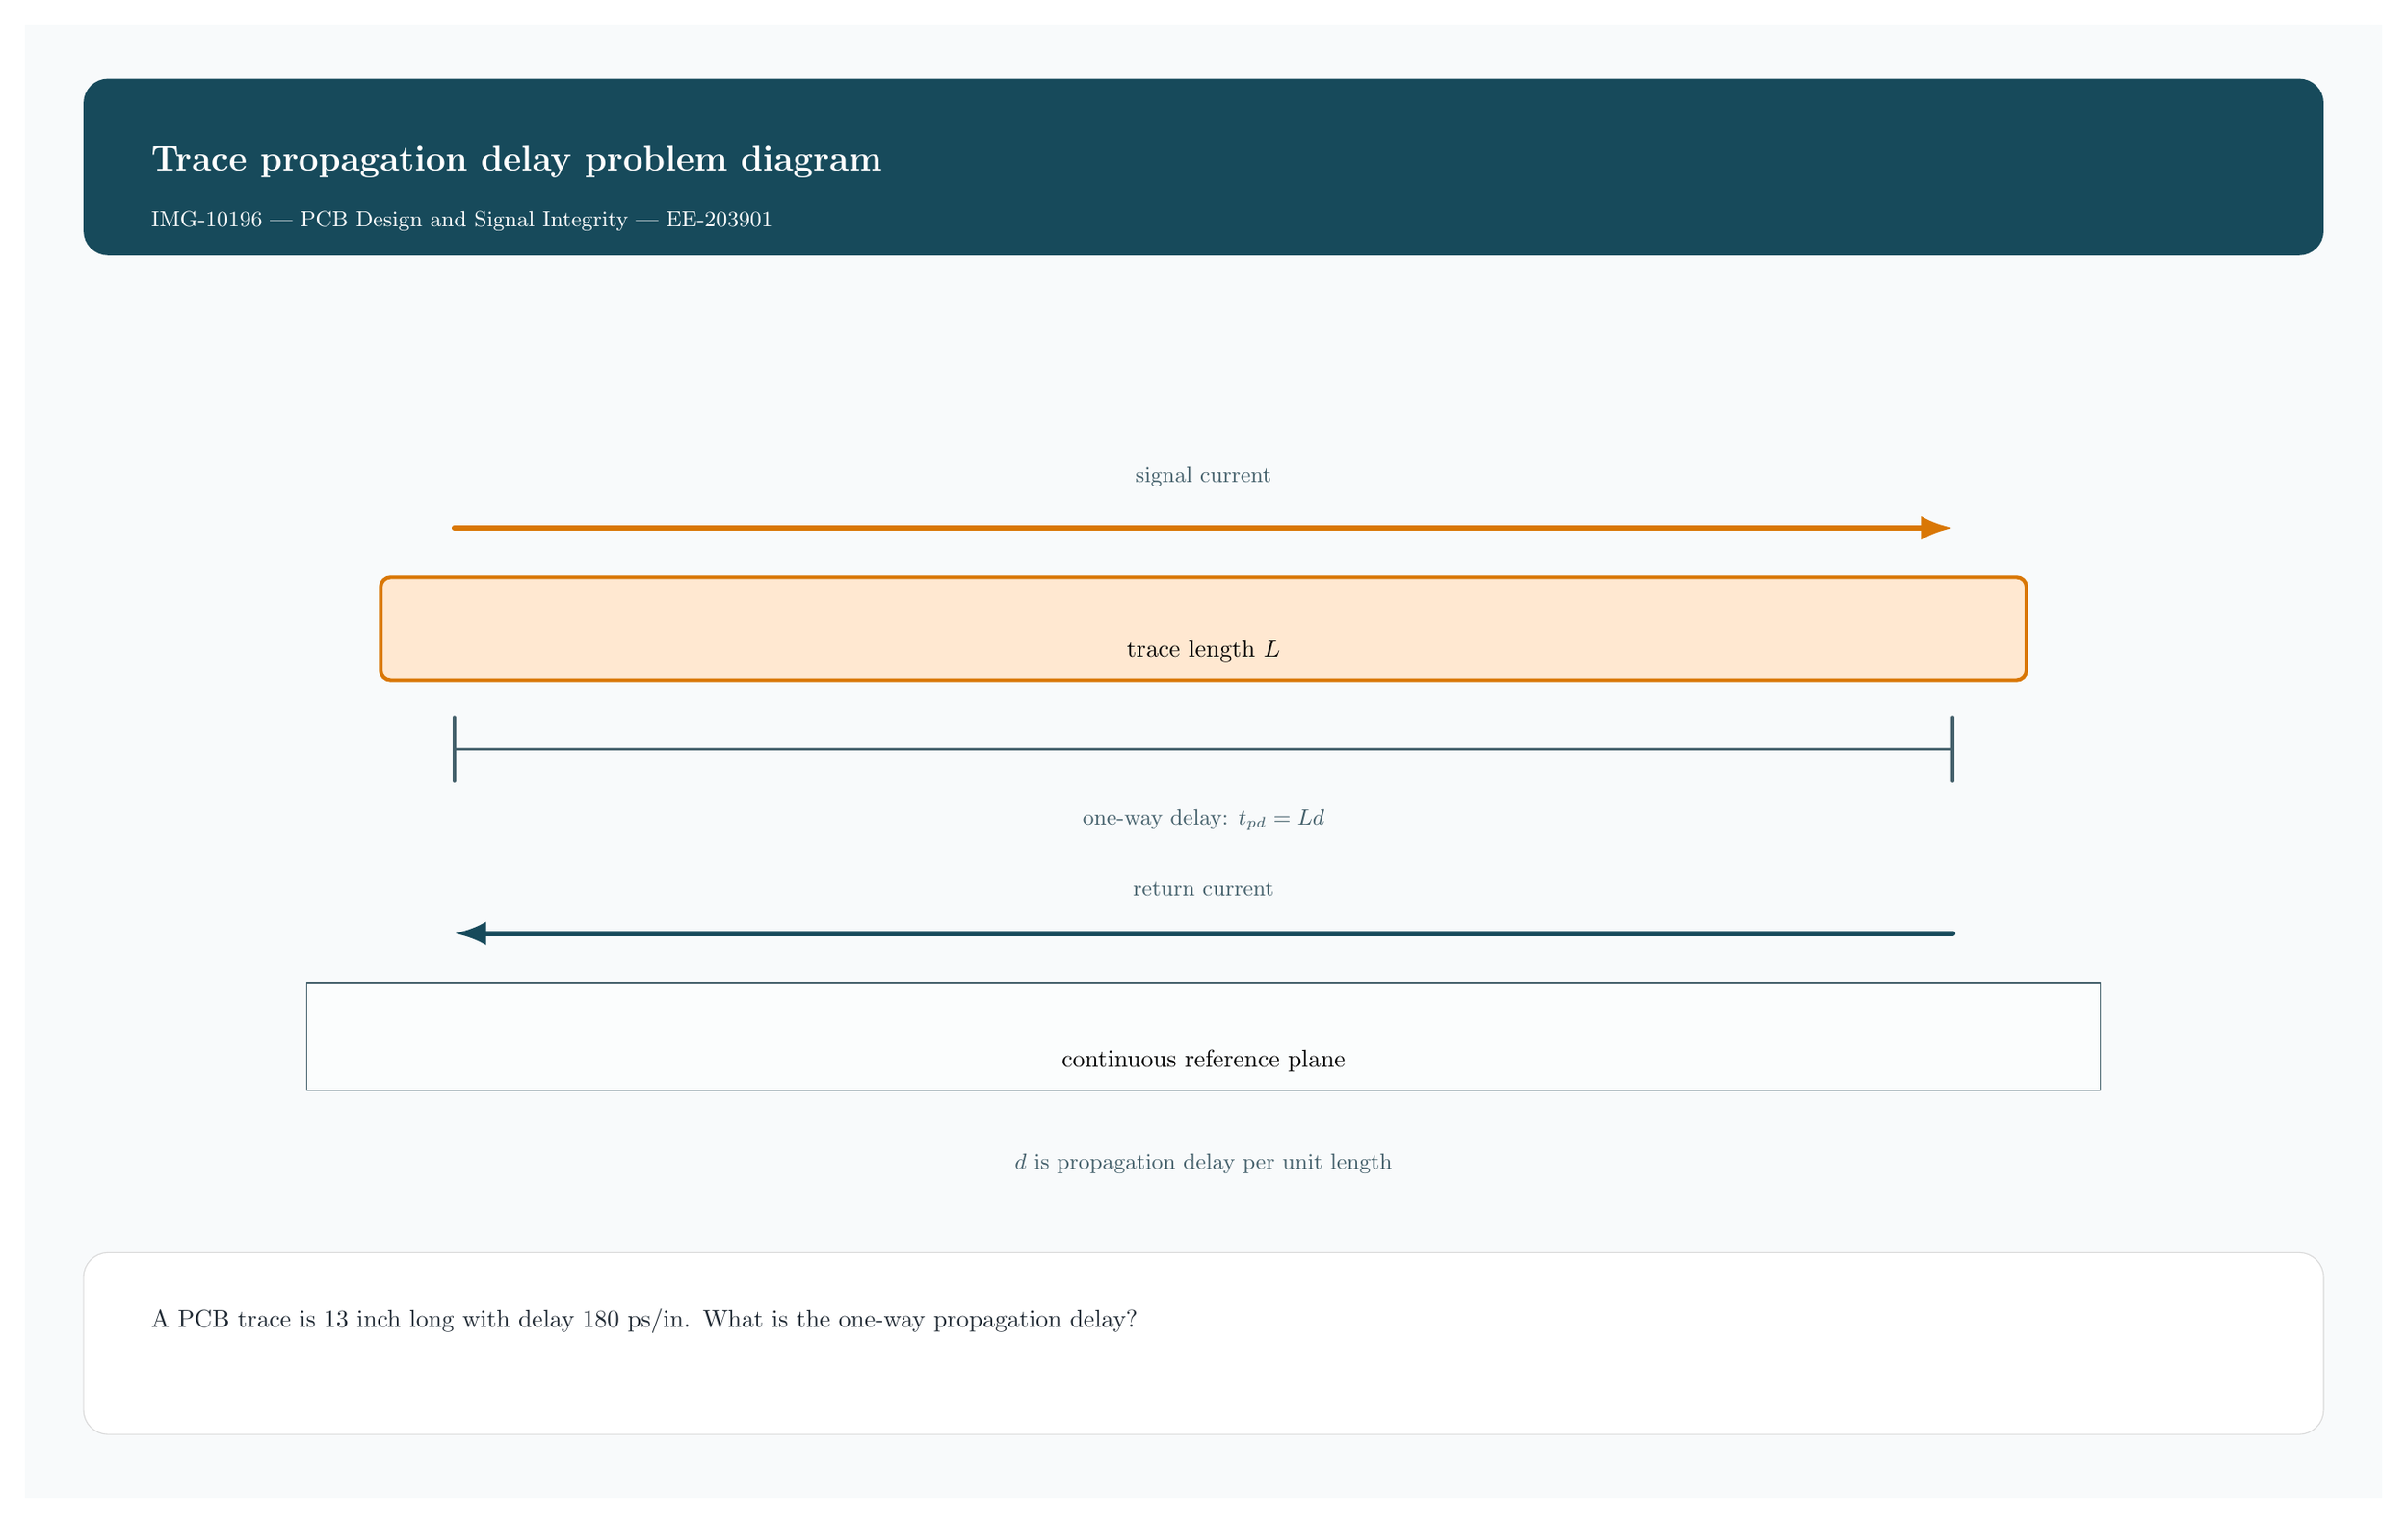
\begin{tikzpicture}[x=1pt,y=-1pt,>=Latex,line cap=round,line join=round]
\path[fill=zyloPaper] (0,0) rectangle (960,600);
\path[fill=zyloTeal,rounded corners=10pt] (24,22) rectangle (936,94);
\node[anchor=west,text=white,font=\bfseries\Large] at (48,56) {Trace propagation delay problem diagram};
\node[anchor=west,text=white!82,font=\small] at (48,80) {IMG-10196 | PCB Design and Signal Integrity | EE-203901};
\tikzset{wire/.style={draw=zyloTeal,line width=2.2pt},thinwire/.style={draw=zyloLine,line width=1.35pt},accent/.style={draw=zyloOrange,line width=2.2pt},box/.style={draw=zyloTealTwo,fill=zyloSoft,line width=1.5pt,rounded corners=8pt}}
\path[draw=zyloOrange,fill=orange!18,rounded corners=4pt,line width=1.5pt] (145,225) rectangle (815,267);
\draw[accent,->] (175,205) -- (785,205); \node[font=\small,text=zyloLine] at (480,184) {signal current};
\node at (480,255) {trace length $L$};
\path[draw=zyloLine,fill=white!80!zyloSoft] (115,390) rectangle (845,434);
\draw[wire,->] (785,370) -- (175,370); \node[font=\small,text=zyloLine] at (480,352) {return current};
\node at (480,422) {continuous reference plane};
\draw[thinwire] (175,295) -- (785,295); \draw[thinwire] (175,282) -- (175,308); \draw[thinwire] (785,282) -- (785,308);
\node[font=\small,text=zyloLine] at (480,324) {one-way delay: $t_{pd}=L d$};
\node[font=\small,text=zyloLine] at (480,464) {$d$ is propagation delay per unit length};
\path[draw=black!15,fill=white,rounded corners=10pt] (24,500) rectangle (936,574);
\node[anchor=west,text width=860pt,align=left,text=zyloInk,font=\normalsize] at (48,528) {A PCB trace is 13 inch long with delay 180 ps/in. What is the one-way propagation delay?};
\end{tikzpicture}
\end{document}
